

\documentclass[twocolumn]{svjour3}       
\journalname{VLDBJ}

%% Font related stuff
%\usepackage{times} 
\usepackage{amsmath} 
\usepackage{amsfonts} 
\usepackage{amssymb} 
%\usepackage{amsthm} 
\usepackage{bold-extra} 
\usepackage[T1]{fontenc} % prettier curly braces in tt mode
\usepackage[scaled]{beramono}
% prettier emptyset
\let\oldemptyset\emptyset
\let\emptyset\varnothing
\DeclareMathOperator{\dist}{dist}

%% Algorithms
\usepackage{listings}
\usepackage[ruled,vlined]{algorithm2e}
\DontPrintSemicolon
\renewcommand{\CommentSty}[1]{\textnormal{#1}}
\SetKwComment{tcp}{$\triangleright$ }{}
\SetVlineSkip{0cm}
\SetAlgoSkip{}


%% others
\usepackage{alltt}
\usepackage{color}
\usepackage{url}
\usepackage[pdftex]{hyperref}
\usepackage{graphicx}
\usepackage{multirow}
\usepackage{blkarray}
\usepackage{balance}
\usepackage{mdframed}

%\usepackage{enumitem}
%\setlist{nolistsep}
%\usepackage{natbib}
%\usepackage[small,compact]{titlesec}
%\titlespacing*{\section}{0pt}{2pt}{1pt}
%\titlespacing*{\subsection}{0pt}{2pt}{1pt}
%\titlespacing*{\subsubsection}{0pt}{2pt}{1pt}
%\titlespacing*{\paragraph}{0pt}{1.75pt}{3pt}
%\usepackage[small,bf,center]{caption}

%% For using smaller font for urls
\makeatletter \def\url@leostyle{\@ifundefined{selectfont}{\def\UrlFont{\sf}}{\def\UrlFont{\scriptsize\ttfamily}}} \makeatother
\urlstyle{leo}

\smartqed  % flush right qed marks
\raggedbottom
%\sloppy 

%% Space savings
%\setlength{\textfloatsep}{0.5\textfloatsep}
%\setlength{\floatsep}{0.5\floatsep}
%\setlength{\intextsep}{0.5\intextsep}
%\setlength{\dbltextfloatsep}{0.5\dbltextfloatsep}
%\setlength{\dblfloatsep}{0.5\dblfloatsep}
%\setlength{\abovecaptionskip}{0.5\abovecaptionskip}
%\setlength{\belowcaptionskip}{0.5\belowcaptionskip}
%\setlength{\footnotesep}{0cm}
%\setlength{\skip\footins}{0.1cm}




\begin{document}
%
% --- Author Metadata here ---
\conferenceinfo{WOODSTOCK}{'97 El Paso, Texas USA}
%\CopyrightYear{2007} % Allows default copyright year (20XX) to be over-ridden - IF NEED BE.
%\crdata{0-12345-67-8/90/01}  % Allows default copyright data (0-89791-88-6/97/05) to be over-ridden - IF NEED BE.
% --- End of Author Metadata ---


\title{Railway: Adaptive Disk Storage for Interaction Graphs}


\numberofauthors{2} 
\author{
\alignauthor
Robert Soul\'{e}\\
       \affaddr{University of Lugano}\\
       \email{robert.soule@usi.ch}  
\alignauthor
Bu\u{g}ra Gedik\\
       \affaddr{Bilkent University}\\
       \email{bgedik@cs.bilkent.edu.tr}
}

\maketitle
\begin{abstract}
  TODO
            
\end{abstract}

% A category with the (minimum) three required fields
\category{H.2.2}{Database Management}{Physical Design - Access methods}
%A category including the fourth, optional field follows...
\category{H.2.4}{Database Management}{Systems - Query Processing}

\terms{Algorithms, Performance}

\keywords{interaction graphs; disk layout; adaptive storage}

\section{Introduction}\label{sec:introduction}

We are living in an ever more connected world, where the data generated by
people, software systems, and the physical world is more accessible than
before and is much larger in volume, variety, and velocity. In many
application domains, such as telecommunications and social media, live data
recording the interactions between people, systems, and the environment is
available for analysis. This data often takes the form of a temporally
evolving graph, where entities are the vertices and the interactions between
them are the edges. We call such graphs \emph{interaction graphs}. 

Data analytics performed on interaction graphs can bring new business insights
and improve decision making. For instance, the graph structure may represent
the interactions in a social network, where finding communities in the graph
can facilitate targeted advertising. In the telecommunications (telco) domain,
call details records (CDRs) can be used to capture the call interactions
between people, and locating closely connected groups of people can be used
for generating promotions. 

Interaction graphs are temporal in nature, and more importantly, they are
append-only. This is in contrast to relationship graphs, which are updated via
insertion and deletion operations. An example of a relationship graph is a
social network capturing the follower-followee relationship among users.
Examples of interactions graphs include CDR graphs capturing calls between
telco customers or mention graphs capturing interactions between users of a
micro-blogging service. The append-only nature of the interaction graphs make
storing them on disk a necessity. Furthermore, the analysis of this historical
interaction data form an important aspect of the analytical landscape.

The ability to efficiently support historical analysis over interaction graphs
require effective solutions for the problem of \emph{data layout} on disk.
Most graph algorithms are characterized by locality of
access~\cite{localityLayout}, which has been taken advantage of co-locating
edges in close proximity within the same disk blocks~\cite{gstoreThesis}. This
ensures that once a disk block is loaded from disk into the main memory
buffers, several edges can be used. The locality of reference is a result of
the traversal-based nature of most of the graph algorithms. 

In interaction graphs, the locality of access is even more pronounced. First, 
the analysis to be performed on the interactions can be restricted to a
temporal view of the graph, such as finding the influential users over a given
week of interactions. This means that edges that are temporally close are to
be accessed together. Second, traversals are again key to many algorithms,
such as connected components, clustering coefficient, PageRank, etc. This
means that edges that are close by in terms of the path between their incident
vertices as well as their timestamps are to be located together with the same
blocks. 

In our earlier work, we introduced an interaction graph database~\cite{gedik14}
that works on this principle of access locality. It proposed a disk
organization that consists of as set of blocks, each containing a list of
\emph{temporal neighbor lists}. A temporal neighborlist contains a head vertex
and a set of incident edges within a given time range. The layout optimizer
aims at bringing together temporal neighborlists that are (i) close in terms
of their temporal ranges, (ii) have many edges between them, and (iii) have
few edges going into temporal neighborlists outside the block.

% Attributes associated with interactions
% I/O inefficiency due to attributes that are not accessed
% Similar to the problem of row vs column stores

Attributes can be stored in two ways, either separately
(e.g., in a relational table), or locally with the temporal neighbor lists. 
If they are stored separately, then the graph database cannot take advantage
of locality optimizations performed for block organization.  As discussed in
Gedik et al.~\cite{gedik14}, the database must go back and forth between the
disk blocks to access the edge attributes.  On the other hand, if attributes
are stored locally in the disk blocks containing the graph structure, then
there can be significant overhead due to disk I/O if only a few attributes are
needed to answer a query.


% Challenges: finding the right partitioning
% what if the access pattern changes over time
% query access patterns are different over different time ranges 

% Solution: railway layout 
% adaptive layout optimization
% algorithms for optimal partitioning
% heuristics & evaluation

Graph databases, and \emph{interaction graph} databases in particular, are a
critical component for many of today's most popular applications.  Graph
databases store entities as vertices, relationships as edges, and have data
associated with either vertices or edges, called \emph{attributes} or
\emph{properties}.  Interaction graphs differ from general graphs in that they
are \emph{append-only}, and edges are assigned a \emph{temporal value}.  Thus,
interaction graphs encode the relationships over time between entities in
their structure, making them ideal for use in social networking,
telecommunications, or modeling the world-wide web.

To query an interaction graph, most algorithms traverse the graph structure to
access the relevant attributes.  Frequently, there are correlations among the
attributes accessed by different queries. For example, queries $q_1$ and $q_5$
might access attributes $a_1$ and $a_2$, while queries $q_2$, $q_3$ and $q_4$
access attributes $a_3$ and $a_4$. Because interaction graphs are temporal,
the co-access correlations for the attributes can vary for different temporal
regions.  Moreover, the co-access correlations might be unknown at the
insertion time, but be discovered later, when the workload is known.

It is widely recognized that query workload and disk layout have a significant
impact on database performance~\cite{alagiannis14,grund10,stonebraker05}.  For
table-based, relational databases, this fact has led database designers to
develop alternative approaches for storage layout: row-oriented storage is
more efficient when queries access many attributes from a small number of
records, and column-oriented storage is more efficient when queries access a
small number of attributes from many records~\cite{stonebraker05}. 
Unfortunately, although interaction graph databases, like relational
databases, are the target of diverse query workloads, there is no clear
correspondence to a row-oriented or column-oriented storage layout.


This paper presents an algorithm for adaptively optimizing disk block storage
for interaction graphs. The key idea behind the approach is a novel storage
scheme, called a \emph{rail layout}.  Initially, attributes are stored with
their neighbor lists in large blocks. Over time, the blocks are split into
smaller-blocks that contain the neighbor lists, but only subsets of the
attributes, depending on the query workload. Intuitively, this is almost like
having two or more graph databases for certain time regions, each containing a
different subset of the attributes, but with a link between them in case a
query needs to access both.

% This points to the need for
% adaptively optimizing the layout (somewhat similar to H2O \cite{alagiannis14}
% and HYRISE~\cite{grund10}).%





\begin{alltt}\scriptsize
- Intro
    - What is an interaction graphs
    - Relationship graphs vs interaction graphs 
        - interactions get big
\end{alltt}

\section{System Overview}\label{sec:system}


\begin{figure}[t]
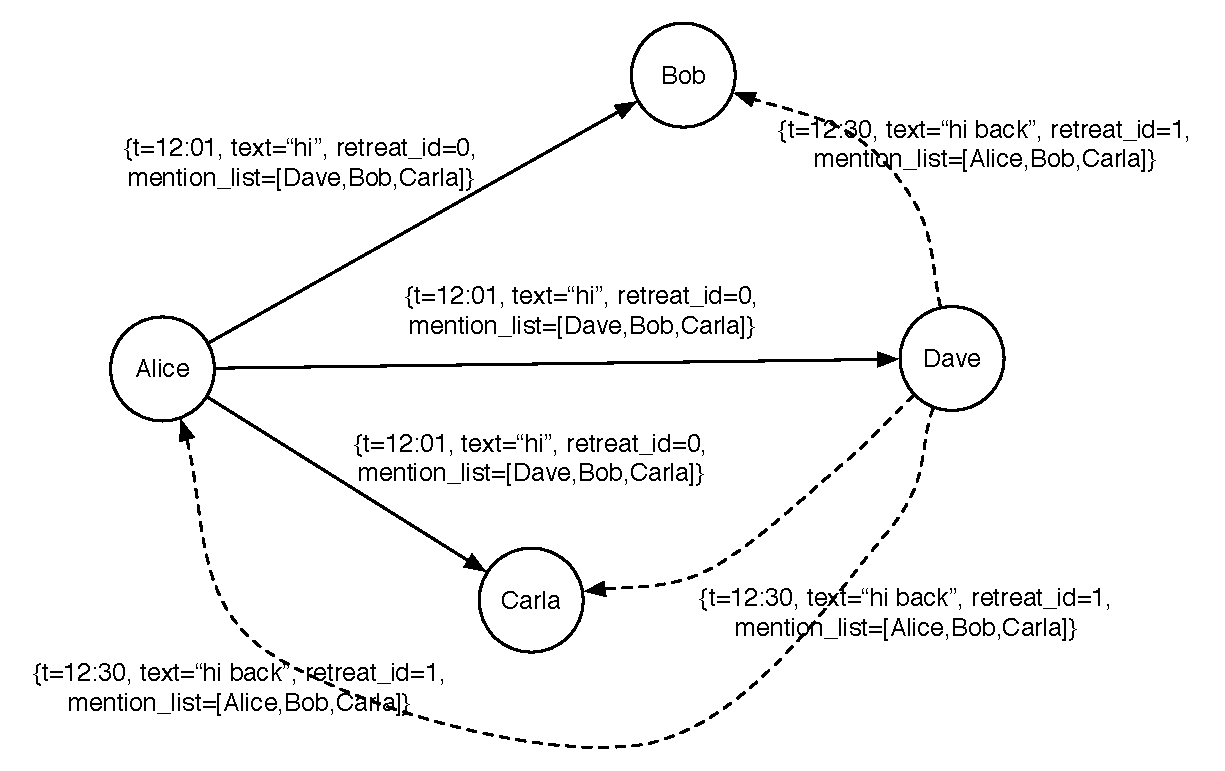
\includegraphics[width=0.9\columnwidth]{figures/example_interaction.pdf} 
 \caption{An example interaction graph for call data records, capturing the
   telephone call interactions among four people. Each edge in the graph is
   associated with attributes for the interaction, including the time the call
   was placed, the duration of the call, the cell phone tower, and the IMEI
   number identifying the device used.}
 \label{fig:example}
 \end{figure}

The design of the railway disk layout builds on our prior work~\cite{gedik14}, 
which organized the disk layout for an interaction graph databases to improve
access locality. The railway layout extends the previous design, by enabling the
system to adapt the layout for changing workloads.

\paragraph*{Motivating Example}
%
To explain the design of the railway layout, we first introduce a small,
motivating example, in Figure~\ref{fig:example}. This figure illustrates an
interaction graph for call data records, capturing the telephone call
interactions among four people. Each edge in the graph is associated with
attributes for the interaction, including the time the call was placed, the
duration of the call, the cell phone tower, and the IMEI number identifying the
device used to place the call. In this example, there were four calls
placed. One of them is a call from Alice to Bob, starting at 13:46. They spoke
for 600 seconds. The call was received by cell phone tower 1, and the Alice's
phone had an IMEI number of 100.

A telecommunications company typically performs various analytics on this
data. For example, for billing purposes, they might want to capture the
duration of all calls. To plan for infrastructure provisioning, they might want
to record a count of the number of calls that each cell phone tower handled.




\begin{figure*}[ht]
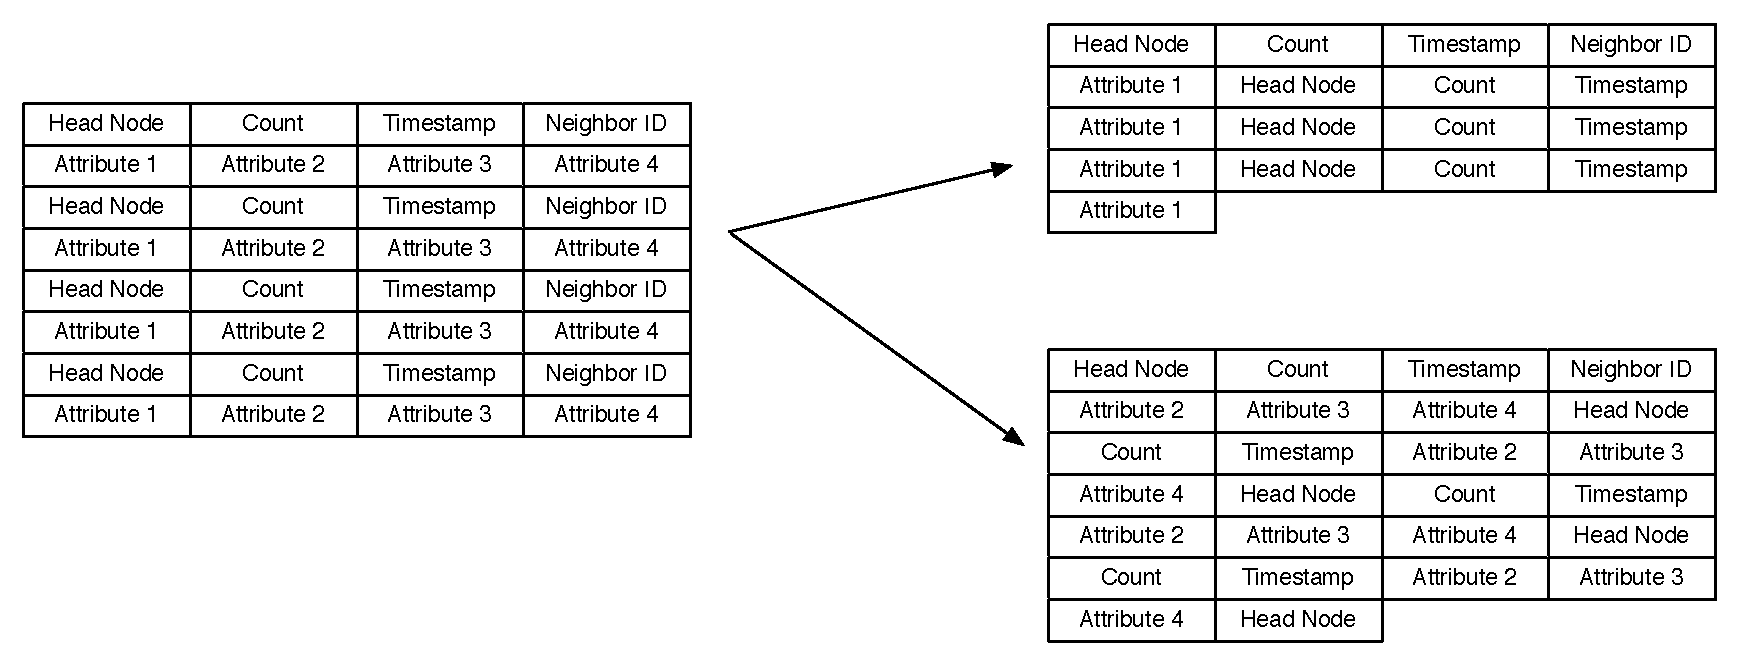
\includegraphics[width=0.9\textwidth]{figures/before_after.pdf} 
 \caption{The standard disk block strorage for an interaction graph, and a
   partitioning into sub-blocks for the railway layout. Each sub-block maintains
 its own copy of the neighbor list, but a subset of the attributes.}
 \label{fig:before_after}
 \end{figure*}

\paragraph*{Storage for Locality}
%
The lefthand side of Figure~\ref{fig:before_after} shows the typical storage for interaction graphs.
Each disk block contains an adjacency list representation of the interaction
graph. The block contains a sequence of vertices, identified by a
\emph{head-node id}, followed by a \emph{count} of the number of neighbors, and
then the neighbor list itself. Each entry in the neighbor list is composed of a
\emph{timestamp}, an \emph{id} for the destination vertex, and the properties
for that edge. 




\paragraph*{Rail Layout}
%




\begin{alltt}\scriptsize
- System overview
    - How interaction graph are currently stored
        - Most of the disk space work is on regular graphs, 
           not interaction graphs. 
        - Approach this as this is the railway, and we built
           on this prior work.
        - Builds on existing work that does not support 
          adaptivity.
    - Introduce the rail layout
    - Add the Figure~\ref{fig:rail_layout}
    - Query model
   - Note that we need to talk here:
    - For the system implementation, we need to add an additional
       index to have a list of partitions for a block
   - We also need to know how attributes are partitioned across sub-blocks 
      for a given time interval.

    - Current layout:
    head vertex (id), num items in neighbor list, 
    for each entry:
        timestamp of edge
        id of other edge of vertex
        any edge properties

\end{alltt}

\begin{figure}[ht]
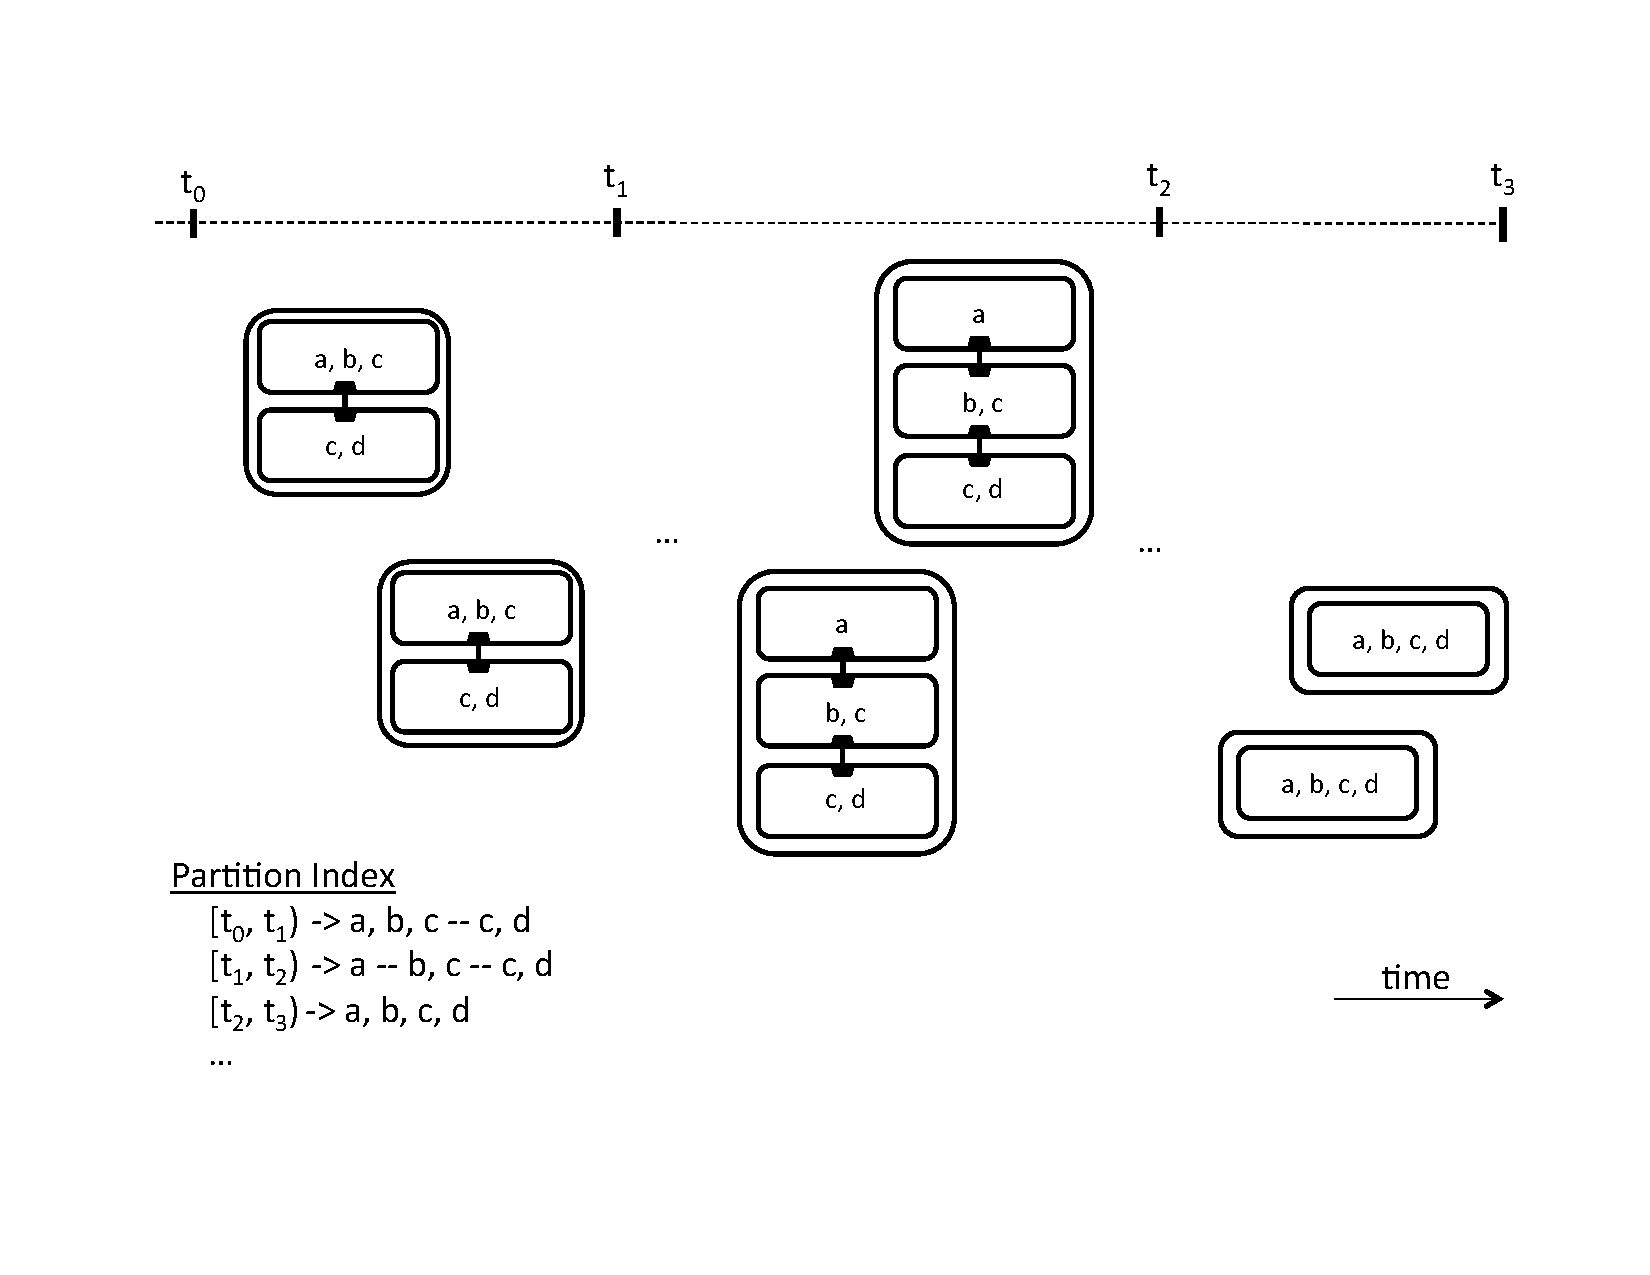
\includegraphics[width=0.9\columnwidth]{figures/rail_layout.pdf} 
 \caption{todo}
 \label{fig:rail_layout}
 \end{figure}

\section{Optimal Railway Design}\label{sec:optimal}  
\noindent
The optimal railway design concerns the partitioning of disk blocks into
sub-blocks such that the query I/O is minimized, while the storage overhead
induced is kept below a desired threshold. This optimization is guided by the
query workload observed by a disk block within a particular time range.

The partitioning of disk blocks into sub-blocks can be \emph{non-overlapping}
or \emph{overlapping}. In the non-overlapping case, the attributes are
partitioned among the sub-blocks with no overlap. In the overlapping case, the
subset of attributes contained within sub-blocks can overlap. In both cases,
the complete graph structure for the block is replicated within the
sub-blocks, which results in a storage overhead.

In both overlapping and non-overlapping partitioning, we trade increased
storage overhead for reduced query I/O cost. In the overlapping case, the
increase in the storage overhead is higher, as some of the attributes are
replicated, in addition to the graph structure. On the other hand, enabling
overlapping attributes is expected to reduce the query I/O (in the extreme
case, there could be one sub-block per query). While the non-overlapping
partitioning scenario is a special case of the  overlapping one, specialized
algorithms can be used to solve the former problem.

In the rest of this section, we first introduce basic notation and then
formulate the overall optimization problem. The modeling of the query I/O and
storage overhead are presented next, which complete the formalization of the
optimal railway design problem.

\subsection{Basic Notation}
\noindent
Let $Q$ be the query workload, where each query $q\in Q$ accesses a set of
attributes $q.A$ and traverses parts of the graph for the time range
$q.T=[q.t_s,q.t_e]$. We denote the set of all attributes as $A$. Given a block
$B$, we denote its time range as $B.T$, which is the union of the time ranges
of its temporal neighborlists. Let $s(a)$ denote the size of an attribute $a$.
We use $c_n(B)$ to denote the number of temporal neighborlists within block
$B$ and $c_e(B)$ to denote the total number of edges in the temporal
neighborlists within the block. We overload the notation for block size and
use $s(B)$ to denote the size of a block $B$. We have: 
\begin{equation}
s(B) = c_e(B) \cdot \Big(16 + \sum_{a\in B.A} s(a)\Big) + c_n(B) \cdot 12  
\end{equation}
Here, $16$ corresponds to the cost of storing the edge id and the timestamp,
and $12$ corresponds to the cost of storing the head vertex ($8$ bytes) plus
the number of entries ($4$ bytes) for a temporal neighborlist. 

Our goal is to create a potentially overlapping partitioning of attributes for
block $B$, resulting in a set of sub-blocks denoted by $\mathcal{P}(B)$. In
other words, we have $\bigcup_{B'\in \mathcal{P}(B)} B'.A = A$. Here,
$\mathcal{P}$ is the partitioning function.

\subsection{Optimization Problem}
\noindent
We aim to find the partitioning function $\mathcal{P}$ that minimizes the query
I/O over $B$, while keeping the storage overhead below a limit, say
$1+\alpha$ times the original. The original corresponds to the case of a single
block that contains all the attributes. Let us denote the query I/O as
$L(\mathcal{P}, B)$ and the storage overhead as $H(\mathcal{P}, B)$,
our goal is to find: 
\begin{equation} 
\mathcal{P} \leftarrow \mbox{argmin}_{\{\mathcal{P}: H(\mathcal{P}(B)) < \alpha\}} L(\mathcal{P},B)
\end{equation}

\subsection{Storage Overhead Formulation}
\noindent
The storage overhead is defined as the additional amount of disk space used to
store the sub-blocks, normalized by the original space needed by a single
block (no partitioning). The storage overhead can be formalized as follows,
for the non-overlapping case:
\begin{equation}
H(\mathcal{P}, B) = (|\mathcal{P}(B)|-1)\cdot\Big(1-\frac{c_e(B)\cdot \sum_{a\in A} s(a)}{s(B)}\Big)
\label{eq:nov}
\end{equation}

Basically, for the non-overlapping case, there is no overhead due to the
attributes, as they are not repeated. However, there is overhead for the block
structure that is repeated for each sub-block. There are $|\mathcal{P}(B)|-1$
such extra sub-blocks, and for each, the contribution to the overhead due to
storing the graph structure is given by $s(B)-c_e(B)\cdot \sum_{a\in A} s(a)$.
Equation~\ref{eq:nov} has one nice feature, that is, it does not depend on the
details of the attribute partitioning, other than the number of partitions. We
make use of this feature, later for the ILP formulation of the problem.

For the general case of a potentially overlapping partitioning, we can
formulate the storage overhead as follows:
\begin{equation}
H(\mathcal{P}, B) = \frac{\sum_{B'\in \mathcal{P}(B)} s(B')}{s(B)} - 1 
\end{equation}

This formulation follows directly from the definition of storage overhead.
While simple, it depends on the details of the partitioning, as $s(B')$ is the
size of a sub-block $B'$, which depends on the list of attributes within the
sub-block.

\subsection{Query I/O Formulation}
\noindent
Let $m$ be a function that maps a query $q$ to the set of sub-blocks that are
accessed to satisfy it for a relevant block $B$ under a given partitioning
$\mathcal{P}$. 

For the case of non-overlapping attributes, the $m$ function lists all the 
sub-blocks whose attributes intersect with those from the query. Formally:
\begin{equation}
m(\mathcal{P}, B, q) = \{B': B'\in \mathcal{P}(B) \wedge q.A \cap B'.A \ne \emptyset\}  
\end{equation}

For the case of overlapping attributes, we use a simple heuristic to define the
set of sub-blocks used for answering the query. Algorithm~\ref{alg:greedyM}
captures it. The basic idea is to start with an empty list of sub-blocks and
greedily add new sub-blocks to it, until all query attributes are covered.  At
each iteration, the sub-block that brings the highest relative marginal gain
is  picked. The relative marginal gain is defined as  the total size of the
attributes from the sub-block that contribute to the query result, relative to
the sub-block size. While computing the marginal gain, attributes that are
already covered by sub-blocks that are selected earlier are not considered.

%
\begin{algorithm}[ht]
\scriptsize
\caption{m-overlapping($\mathcal{P}, B, q$)}
\label{alg:greedyM}
\KwData{$\mathcal{P}$: partitioning function, $B$: block, $q$: query}
$S\leftarrow \emptyset; R\leftarrow \emptyset$ \tcp*{Selected attributes; Resulting sub-blocks}
\While(\tcp*[f]{While unselected attributes remain}){$S \subset q.A$}{
  $B' \leftarrow \mbox{argmax}_{B'\in\mathcal{P}(B)\setminus R} \sum_{a\in B'.A \cap q.A \setminus S} \frac{c_e(B') \cdot s(a)}{s(B')}$
  $S \leftarrow S \cup B'.A$\tcp*{Extend the selected attributes}
  $R\leftarrow R \cup B'$\tcp*{Extend the selected sub-blocks}
}
\Return R \tcp*{Final set of sub-blocks covering the query attributes}
\end{algorithm} 

HERE
The query I/O cost for a block is then given by:
\begin{equation}
L(\mathcal{P}, B) = \sum_{q\in Q} w(q)\cdot\mathbf{1}(q.T \cap B.T \neq \emptyset) \cdot \sum_{B'\in m(\mathcal{P}, B, q)} \!\!s(B')
\end{equation}

Here, $w(q)$ represents the query weight.



\section{ILP Solution}\label{sec:ilp}

\section{Heuristic Solution}\label{sec:heuristic}


\begin{alltt}
- Talk about the scalability of the optimal solution
- Do we have a running time?
- Introduce a heuristic approximation approach
\end{alltt}

\subsection{Non-Overlapping Partitions}\label{subsec:nov-heuristic}
\noindent


\paragraph*{Approach$\,$}
TODO

\begin{algorithm}[ht]
\scriptsize
\caption{Algorithm for partitioning blocks into sub-blocks with non-overlapping attributes.}
\label{alg:non-overlappingP}
\KwData{$B$: block, $Q$: set of queries}
$c^*\leftarrow \infty$ \tcp*{Lowest cost over all \# of partitions}
\For(\tcp*[f]{For each possible \# of partitions}){$k=1$ to $|A|$}{
   $R[i]\leftarrow \emptyset, \forall i\in [1..k]$ \tcp*{Initialize partitions}
   \For(\tcp*[f]{For each attribute}){$a \in A$\textnormal{, in decr.\/ order of }$f(a)$}{
      $c\leftarrow \infty$ \tcp*{Lowest cost over all assignments}  
      $j\leftarrow -1$ \tcp*{Best partition assignment}
      \For(\tcp*[f]{For each partition assignment}){$i\in [1..k]$} {
         $R[i]\leftarrow R[i] \cup \{a\}$\tcp*{Assign attribute}
         \If(\tcp*[f]{If query cost is lower}){$L(R, B, Q)<c$}{
            $c\leftarrow L(R, B, Q)$\tcp*{Update the lowest cost}
            $j\leftarrow i$\tcp*{Update the best partition}
         }
         $R[i]\leftarrow R[i] \setminus \{a\}$\tcp*{Un-assign attribute}
      }
      $R[j]\leftarrow R[j] \cup \{a\}$\tcp*{Assign to best partition}
   }
   \lIf(\tcp*[f]{If solution infeasible}){$H(R, B, Q)>\alpha$}{\textbf{break}}
   \If(\tcp*[f]{If solution has lower cost}){$L(R, B, Q)<c^*$}{
     $c^* \leftarrow L(R, B, Q)$\tcp*{Update the lowest cost}
     $\mathcal{P}(B)\leftarrow R$\tcp*{Update the best partitioning}
   } 
}
\Return $\mathcal{P}(B)$ \tcp*{Final set of sub-blocks}
\end{algorithm} 


\subsection{Overlapping Partitions}\label{subsec:ov-heuristic}
\noindent


\paragraph*{Approach$\,$} We start the algorithm with a   partitioning based
on what queries we have seen. Every query gets its own sub-block. This is the
``ideal'' partitioning, because the I/O cost would be minimized for every
query that we would have seen. The algorithm iteratively combines the two
partitions that are closest together.  After each combination of partitions,
the algorithm calculate the storage overhead for the partitioning. The
algorithm stops when the  storage cost is below some specified threshold.  The
result is the block partitioning.

\begin{algorithm}[ht]
\scriptsize
\caption{Algorithm for partitioning blocks into sub-blocks with overlapping attributes.}
\label{alg:overlappingP}
\KwData{$B$: block, $Q$: set of queries}
$\mathcal{P}(B) \leftarrow \{q.A: q\in Q\}$ \tcp*{Each query gets its own sub-block}
\While(\tcp*[f]{Until storage overhead is below $\alpha$}){$H(\mathcal{P},B) > \alpha$}{
  $c^{*}\gets \infty $ \tcp*{Lowest cost over all sub-block pairs}
  $(b_x,b_y)\gets (\emptyset,\emptyset)$ \tcp*{Sub-block pair with the lowest cost}
  \For(\tcp*[f]{For each pair of blocks}){$\{b_i,b_j\}\in\mathcal{P}(B)$}{
    $\mathcal{P'}(B) \leftarrow \mathcal{P}(B) \setminus \{b_i, b_j\} \cup \{b_i \cup b_j\}$\\
    $c\gets \frac{L(\mathcal{P}',B,Q)-L(\mathcal{P},B,Q)}{H(\mathcal{P},B)-H(\mathcal{P}',B)}$\tcp*{Cost of merge}
    \If(\tcp*[f]{Cost is lower}){$c<c^{*}$}{
        $c^{*}\gets c$\tcp*{Update the lowest cost}
        $(b_x,b_y)\gets (b_i,b_j)$\tcp*{Update the best pair}
    }
  }
  $\mathcal{P}(B) \leftarrow \mathcal{P}(B) \setminus \{b_x, b_y\} \cup \{b_x \cup b_y\}$ \\
}
\Return $ \mathcal{P}(B)$  \tcp*{Final set of sub-blocks}
\end{algorithm} 

\begin{verbatim}
1) RunningTimeVsNumAttributes:
  x axis: # attributes
  y axis: running time
  series: optimal-nov, optimal-ov, heuristic-nov, heuristic-ov

2) RunningTimeVsNumQueryKinds:
  x axis: num query kinds
  y axis: running time
  series: optimal-nov, optimal-ov, heuristic-nov, heuristic-ov

3) QueryIOVsNumAttributes:
  x axis: # attributes
  y axis: query IO
  series: optimal-nov, optimal-ov, heuristic-nov, heuristic-ov, single-block, per-attribute

4) StorageOverheadVsNumAttributes:
  x axis: # attributes
  y axis: storage overhead
  series: optimal-nov, optimal-ov, heuristic-nov, heuristic-ov, single-block, per-attribute
  
5) QueryIOVsStorageOverheadThreshold:
  x axis: query overhead threshold
  y axis: query IO
  series: optimal-nov, optimal-ov, heuristic-nov, heuristic-ov, single-block, per-attribute

6) StorageOverheadVsStorageOverheadThreshold:
  x axis: query overhead threshold
  y axis: storage overhead
  series: optimal-nov, optimal-ov, heuristic-nov, heuristic-ov, single-block, per-attribute

7) QueryIOVsNumQueryKinds:
  x axis: num query kinds
  y axis: query IO
  series: optimal-nov, optimal-ov, heuristic-nov, heuristic-ov, single-block, per-attribute

8) StorageOverheadVsNumQueryKinds:
  x axis: num query kinds
  y axis: storage overhead
  series: optimal-nov, optimal-ov, heuristic-nov, heuristic-ov, single-block, per-attribute

9) QueryIOVsAttributeSizeSkew:
  x axis: attribute size skew
  y axis: query IO
  series: optimal-nov, optimal-ov, heuristic-nov, heuristic-ov, single-block, per-attribute

10) StorageOverheadVsAttributeSizeSkew:
  x axis: attribute size skew
  y axis: storage overhead
  series: optimal-nov, optimal-ov, heuristic-nov, heuristic-ov, single-block, per-attribute

11) QueryIOVsQueryLength:
  x axis: mean query length
  y axis: query IO
  series: optimal-nov, optimal-ov, heuristic-nov, heuristic-ov, single-block, per-attribute

12) StorageOverheadVsQueryLength:
  x axis: mean query length
  y axis: storage overhead
  series: optimal-nov, optimal-ov, heuristic-nov, heuristic-ov, single-block, per-attribute

13) QueryIOVsQueryFreqSkew:
  x axis: query freq skew
  y axis: query IO
  series: optimal-nov, optimal-ov, heuristic-nov, heuristic-ov, single-block, per-attribute

14) StorageOverheadVsQueryFreqSkew:
  x axis: query freq skew
  y axis: storage overhead
  series: optimal-nov, optimal-ov, heuristic-nov, heuristic-ov, single-block, per-attribute
\end{verbatim}
\section{Related Work}

\begin{alltt}\scriptsize
Gedik et al.~\cite{gedik14}
H2O \cite{alagiannis14}
HYRISE~\cite{grund10}
Bornea et al.~\cite{bornea13}
\end{alltt}


\section{Conclusion}\label{sec:conclusion}



\bibliographystyle{abbrv}
\bibliography{paper}  
\end{document}
